\section{پروژه پنجم: تشخیص وسایل نقلیه با \lr{YOLOv8}}
در این پروژه، هدف آموزش و تنظیم دقیق (\lr{Fine-tuning}) شبکه‌ی پیچشیِ \lr{YOLO} برای تشخیص ۵ کلاس مختلف از وسایل نقلیه (خودرو، دوچرخه، اتوبوس، کامیون و موتورسیکلت) است. با توجه به نیاز مسئله به تعادل میان سرعت پردازش (\lr{Inference Speed}) و دقت تشخیص، از معماری پیشرفته‌ی \lr{YOLOv8} استفاده شده است. این نسخه با بهره‌گیری از مکانیزم \lr{Anchor-free} (بدون نیاز به لنگرهای ازپیش‌تعریف‌شده)، انعطاف‌پذیری بسیار بالایی در تشخیص اهداف با ابعاد بسیار متفاوت (مانند یک دوچرخه در کنار یک اتوبوس) از خود نشان می‌دهد.

\vspace{0.4cm}
\subsection{آماده‌سازی محیط و پایشگر آموزش (\lr{Monitoring})}
به‌منظور ثبت دقیق روند آموزش، رهگیری متریک‌های ارزیابی و استخراج خودکار نمودارها جهت تحلیل‌های بعدی، از پلتفرم یکپارچه‌ی \lr{Weights \& Biases (WandB)} استفاده گردید.

\begin{stepbox}
\field{راه‌اندازی اولیه و اتصال به \lr{WandB}}{
ابتدا کتابخانه‌های \lr{\texttt{ultralytics}} و \lr{\texttt{wandb}} در محیط \lr{Google Colab} نصب و پیکربندی شدند. پس از احراز هویت از طریق \lr{API Key} اختصاصی، یک جریان دادهِ بی‌درنگ (\lr{Real-time Stream}) بین محیط آموزش و سرورهای \lr{WandB} برقرار شد. این ابزار به ما اجازه می‌دهد تا نوسانات تابع زیان (\lr{Loss})، تغییرات نرخ یادگیری (\lr{Learning Rate}) و معیارهای ارزیابی نظیر \lr{mAP} را در تک‌تک دوره‌های آموزشی (\lr{Epochs}) رصد کرده و در صورت بروز مشکلاتی نظیر محوشدگی گرادیان (\lr{Vanishing Gradient})، فرآیند را به‌سرعت متوقف و اصلاح نماییم.
}
\end{stepbox}

\vspace{0.4cm}
\subsection{آماده‌سازی پایگاه داده و منطق برچسب‌گذاری}
دیتاست مورد استفاده در این پروژه شامل تصاویر متنوعی از وسایل نقلیه در شرایط نوری، زوایا و پس‌زمینه‌های گوناگون است. فرآیند برچسب‌گذاری (\lr{Labeling}) شامل ترسیم دقیق کادرهای احاطه‌گر (\lr{Bounding Boxes}) برای ۵ کلاسِ هدف انجام گرفت و خروجی‌ها به فرمت استاندارد \lr{YOLO} (مختصات نرمال‌شده‌ی مرکز، عرض و ارتفاع کادر) تبدیل شدند.

\begin{stepbox}
\field{تقسیم‌بندی استاندارد داده‌ها}{
برای حصول اطمینان از آموزش اصولی و سنجش دقیقِ تعمیم‌پذیریِ شبکه روی داده‌های دیده نشده، مجموعه‌داده با یک توزیع تصادفی به سه زیرمجموعه‌ی مجزا تقسیم گردید:
\begin{itemize}
    \item \textbf{داده‌های آموزش (\lr{Train - 70\%}):} قلب تپنده‌ی فرآیند یادگیری؛ داده‌هایی که در مسیر رو به جلو (\lr{Forward Pass}) پردازش شده و خطای آن‌ها از طریق الگوریتم پس‌انتشار (\lr{Backpropagation}) برای به‌روزرسانی وزن‌ها استفاده می‌شود.
    \item \textbf{داده‌های اعتبارسنجی (\lr{Validation - 20\%}):} داده‌هایی ایزوله از فرآیند آپدیت وزن‌ها، که در پایان هر اپوک برای ارزیابی عملکرد مدل و جلوگیری از پدیده‌ی حفظ‌کردن داده‌ها استفاده می‌شوند.
    \item \textbf{داده‌های آزمون (\lr{Test - 10\%}):} داده‌های کاملاً بکر جهت ارزیابی نهایی و شبیه‌سازی عملکرد مدل در محیط عملیاتی واقعی.
\end{itemize}
}
\end{stepbox}

\vspace{0.4cm}
\subsection{آموزش شبکه‌ها و ارزیابی کمی مدل‌ها}
به‌منظور یافتن بهینه‌ترین معماری برای این مجموعه داده‌ی خاص، رویکرد یادگیری انتقالی (\lr{Transfer Learning}) اتخاذ شد. سه نسخه‌ی مختلف از خانواده‌ی \lr{YOLOv8} (شامل \lr{Small, Medium, Large}) با وزن‌های ازپیش‌آموزش‌دیده روی دیتاست عظیم \lr{COCO} بارگذاری شدند. 

در تمامی آزمایش‌ها، بهینه‌ساز \lr{AdamW} (ترکیب \lr{Adam} با \lr{Weight Decay} برای کنترل پیچیدگی وزن‌ها) با اندازه‌ی تصویر ۶۴۰ پیکسل و به مدت ۳۰ اپوک مورد استفاده قرار گرفت. اندازه‌ی دسته (\lr{Batch Size}) برای مدل \lr{Large} به دلیل محدودیت‌های حافظه‌ی گرافیکی (\lr{VRAM}) به ۸ کاهش یافت.

\begin{stepbox}
\field{خلاصه نتایج و مقایسه عملکرد معماری‌ها}{
ارزیابی نهایی مدل‌ها روی مجموعه‌ی اعتبارسنجی با دو معیار سخت‌گیرانه‌ی \lr{mAP@50} (دقت با حد آستانه اشتراک ۵۰ درصد) و \lr{mAP@50-95} (میانگین دقت در آستانه‌های مختلف) انجام شد:
\begin{itemize}
    \item \textbf{مدل \lr{YOLOv8 Small (s)}:} ۱۱.۱ میلیون پارامتر | \lr{mAP@50}: \textbf{$84.6\%$} | \lr{mAP@50-95}: \textbf{$74.3\%$}
    \item \textbf{مدل \lr{YOLOv8 Medium (m)}:} ۲۵.۸ میلیون پارامتر | \lr{mAP@50}: $68.2\%$ | \lr{mAP@50-95}: $59.8\%$
    \item \textbf{مدل \lr{YOLOv8 Large (l)}:} ۴۳.۶ میلیون پارامتر | \lr{mAP@50}: $75.4\%$ | \lr{mAP@50-95}: $63.9\%$
\end{itemize}
}
\end{stepbox}

\begin{tipbox}[تحلیل آماری: ظرفیت شبکه در برابر حجم داده]
برخلاف تصور رایج که "مدل بزرگ‌تر همواره نتایج بهتری تولید می‌کند"، مشاهدات ما نشان می‌دهد که مدل سبکِ \lr{Small} با اختلاف حدود ۱۶ درصد از مدل \lr{Medium} بهتر عمل کرده است. 
دلیل علمی این پدیده، عدم تناسب میان \textbf{ظرفیت بازنمایی (\lr{Representational Capacity}) مدل} و \textbf{حجم داده‌های آموزشی} است. مدل‌های مدیوم و لارج با ده‌ها میلیون پارامتر، به داده‌های فراوانی نیاز دارند تا الگوهای عمومی را بیاموزند. در مواجهه با دیتای محدودِ این پروژه، این مدل‌های عظیم به‌سرعت دچار بیش‌برازش (\lr{Overfitting}) شده و به‌جای درک ویژگی‌های ظاهری وسایل نقلیه، صرفاً نویزها و مشخصات خاصِ عکس‌های آموزشی را حفظ کرده‌اند. در نتیجه، هنگام مواجهه با عکس‌های اعتبارسنجی، دچار افت شدید دقت شده‌اند.
\end{tipbox}

\vspace{0.4cm}
\subsection{تحلیل بصری روند آموزش و کالبدشکافی توابع زیان}
برای اعتبارسنجی تئوری مطرح شده در بخش قبل، نمودارهای استخراج‌شده از \lr{WandB} مورد ارزیابی دقیق قرار گرفت. در \lr{YOLOv8} از سه تابع زیان اصلی استفاده می‌شود: \lr{box\_loss} (برای دقت مختصات کادر)، \lr{cls\_loss} (برای دقت تشخیص کلاس) و \lr{dfl\_loss} (برای ظرافت در تشخیص لبه‌های مرزی شیء).

\begin{notebox}[تحلیل رفتار دینامیک شبکه‌ها پیش از بررسی نمودارها]
با بررسی خروجی‌ها، دو الگوی کاملاً متمایز قابل شناسایی است:
\begin{itemize}
    \item \textbf{همگرایی پایدار (\lr{مدل Small}):} زیان دسته‌بندی و زیان کادر با شیب ملایم رو به کاهش هستند و معیارهای دقت به‌سرعت بازیابی شده و به پایداری رسیده‌اند.
    \item \textbf{فروپاشی مقطعی (\lr{مدل‌های Medium و Large}):} یک فاجعه‌ی یادگیری در بازه‌ی اپوک‌های ۱۰ تا ۲۰ رخ داده است. خطای اعتبارسنجیِ کلاس در مدل مدیوم به عدد نجومی ۲۰,۰۰۰ جهش کرده و دقت مستقیماً روی صفر سقوط می‌کند. این پرش‌ها (\lr{Spikes}) نشان‌دهنده‌ی ناپایداری شدید در فضای وزن‌ها به دلیل ظرفیت بیش‌ازحدِ شبکه نسبت به داده‌ها است.
\end{itemize}
\end{notebox}

در شکل \ref{fig:all_models_charts}، این تفاوت رفتار به‌وضوح به تصویر کشیده شده است. برای جلوگیری از اشغال فضای بیش‌ازحد صفحه، نمودارها به‌صورت فشرده در کنار یکدیگر قرار گرفته‌اند.

\begin{figure}[ht!]
    \centering
    \begin{subfigure}{0.48\textwidth}
        \centering
        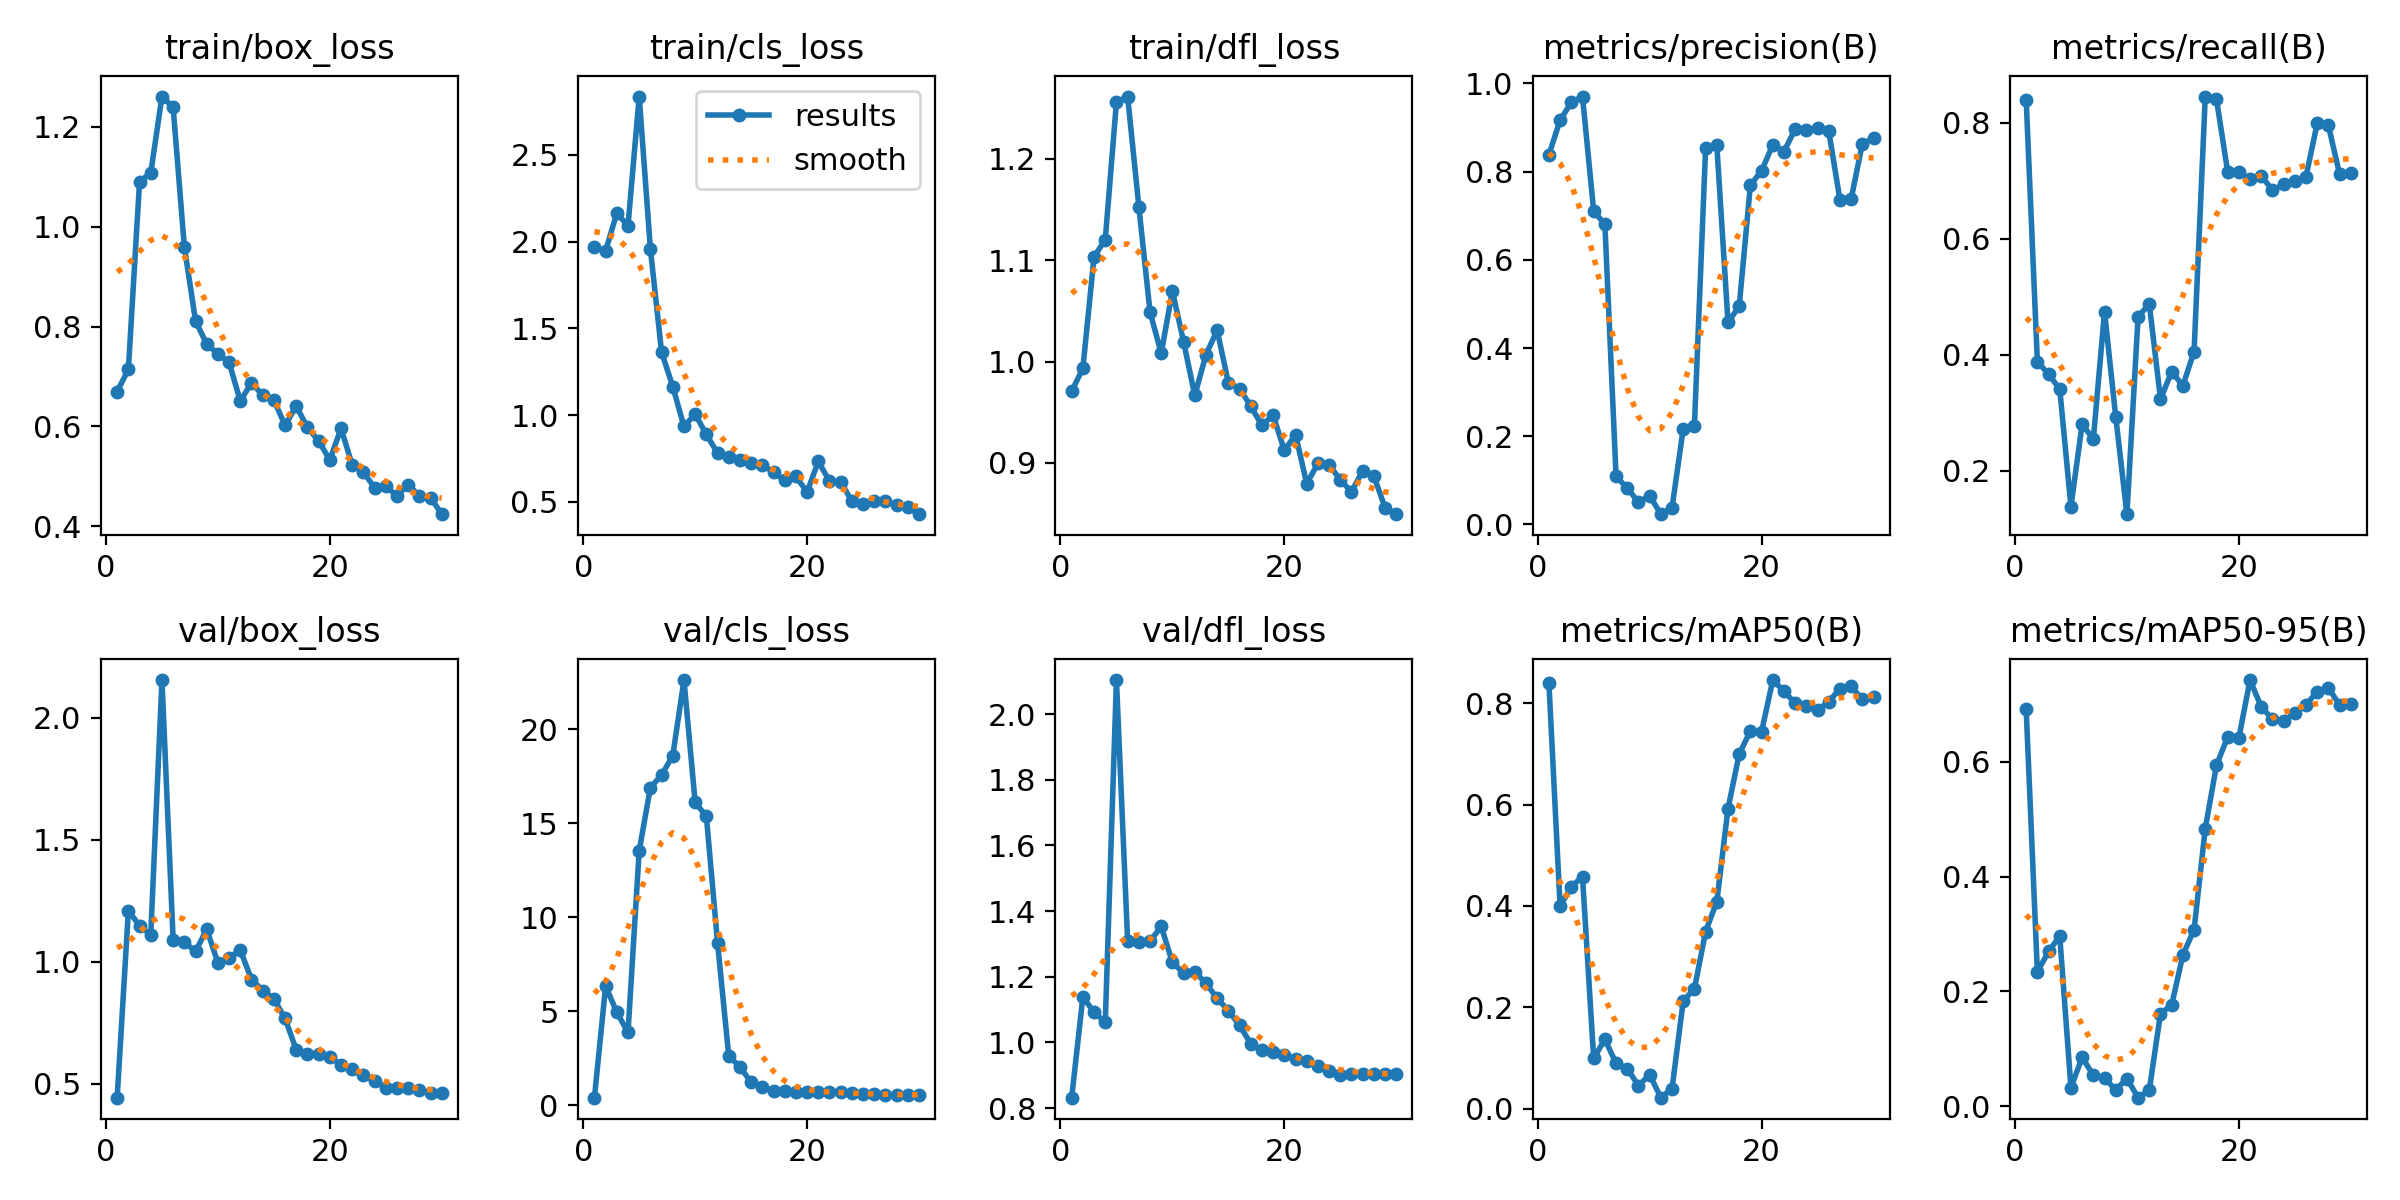
\includegraphics[width=\textwidth]{images/wandb_small.png}
        \caption{مدل \lr{Small} (همگرایی پایدار)}
    \end{subfigure}
    \hfill
    \begin{subfigure}{0.48\textwidth}
        \centering
        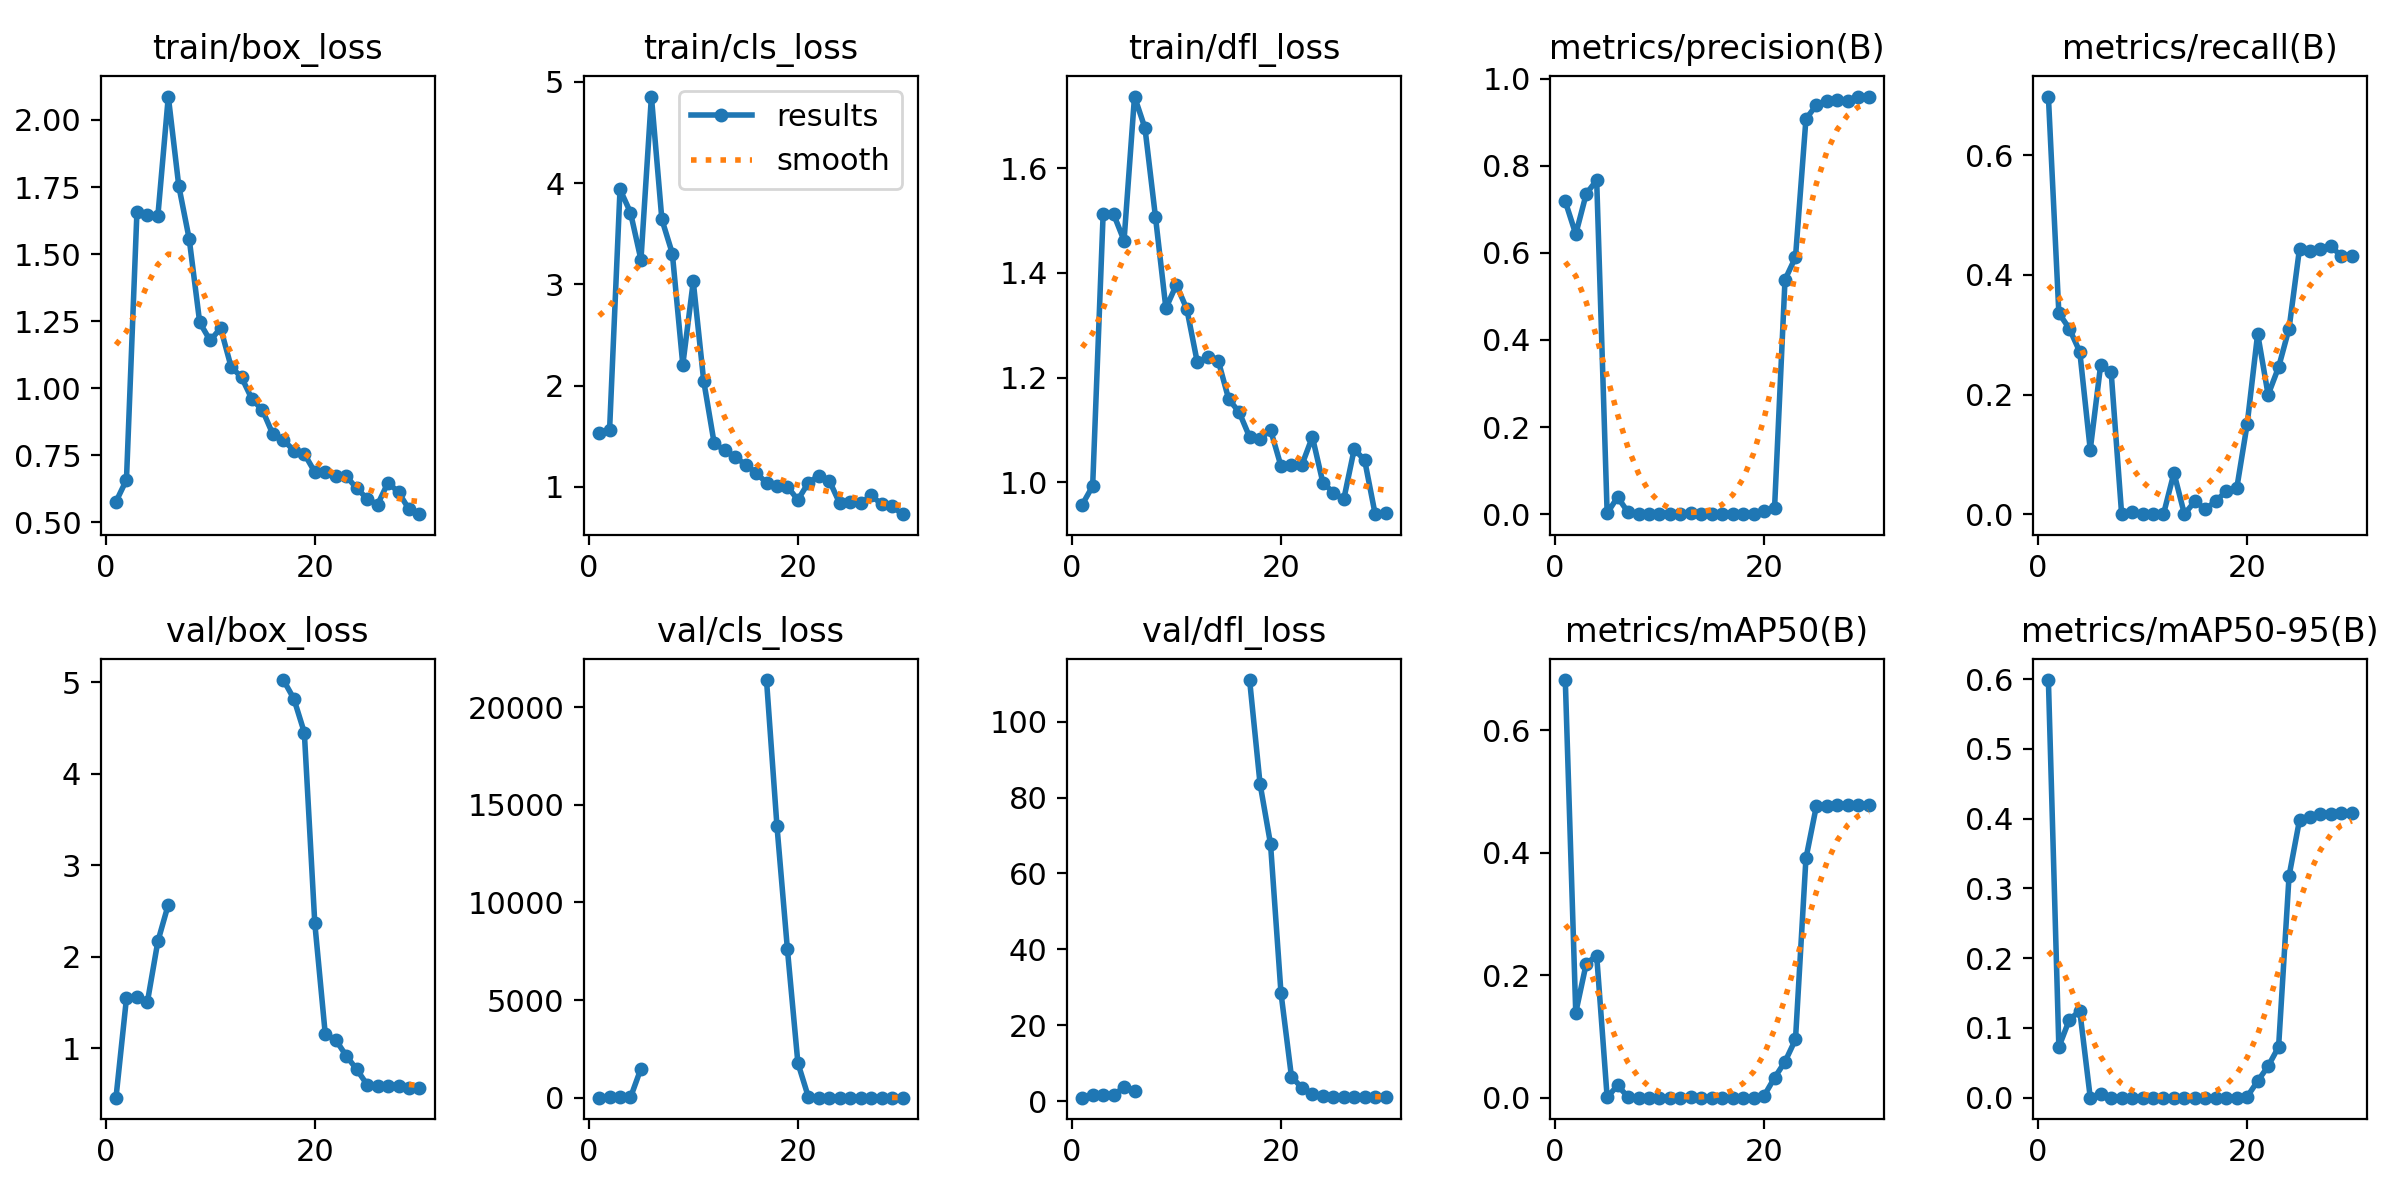
\includegraphics[width=\textwidth]{images/medium_model.png}
        \caption{مدل \lr{Medium} (فروپاشی و جهش خطا)}
    \end{subfigure}
    
    \vspace{0.4cm}
    \begin{subfigure}{0.48\textwidth}
        \centering
        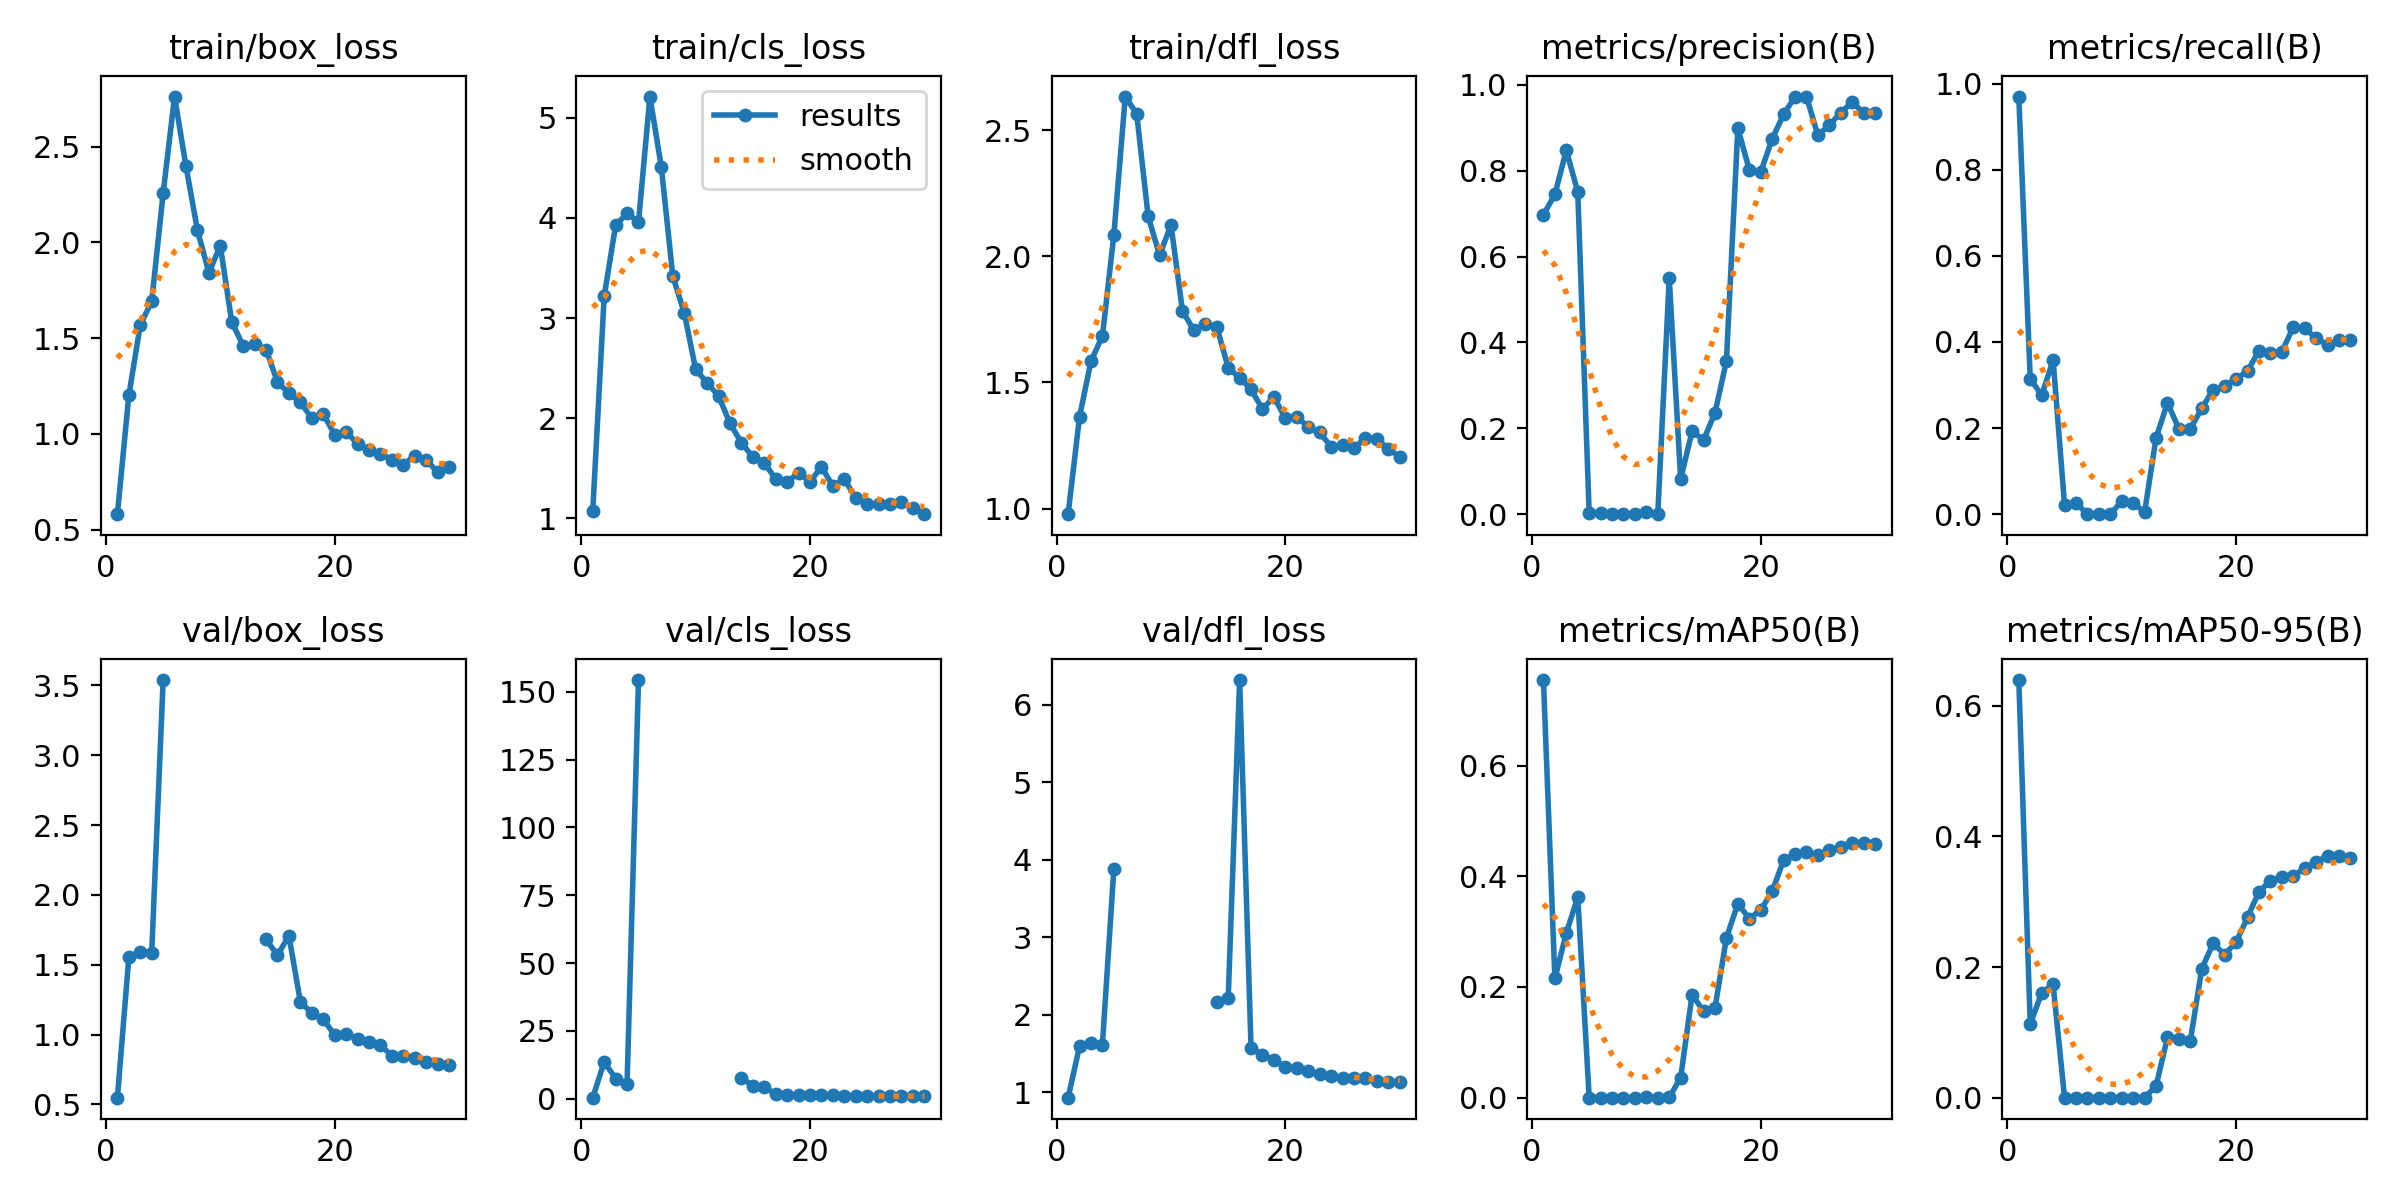
\includegraphics[width=\textwidth]{images/large_model.png}
        \caption{مدل \lr{Large} (نوسانات آشوبناک)}
    \end{subfigure}
    \caption{مقایسه رفتار دینامیک سه معماری در طول ۳۰ اپوک.}
    \label{fig:all_models_charts}
\end{figure}

\vspace{0.4cm}
\subsection{خروجی‌های تصویری (\lr{Inference}) و نتیجه‌گیری نهایی}
پس از اثبات تئوریک و بصریِ برتریِ معماری \lr{Small} برای این مسئله، در این مرحله عملکرد مدلِ منتخب روی داده‌های نادیده‌ی اعتبارسنجی مورد آزمایش قرار می‌گیرد. 
مدل با اعمال الگوریتم سرکوب غیربیشینه (\lr{Non-Maximum Suppression - NMS}) کادرهای تکراری را فیلتر کرده و تنها محتمل‌ترین محدوده‌ها را نگه می‌دارد. نتیجه‌ی این عملیات در شکل \ref{fig:val_pred} قابل مشاهده است.

\begin{figure}[ht!]
    \centering
    
\includegraphics[width=0.75\textwidth]{images/val_batch0_pred.jpg}
    \caption{نمونه‌ای از استنتاج موفق شبکه در شناسایی وسایل نقلیه و اعمال \lr{NMS}}
    \label{fig:val_pred}
\end{figure}

همان‌طور که در تصویر \ref{fig:val_pred} مشاهده می‌شود، شبکه با وجود پس‌زمینه‌های شلوغ، توانسته است وسایل نقلیه را با درصد اطمینان بالا (\lr{Confidence Score}) مکان‌یابی و در کلاس صحیح دسته‌بندی نماید. 

\begin{tipbox}[نتیجه‌گیری راهبردی]
این پروژه به شکل تجربی اثبات نمود که در محیط‌های عملیاتی و در صورت عدم دسترسی به مجموعه‌داده‌های عظیم در مقیاس میلیون‌ها تصویر، انتخاب یک شبکه‌ی چابک با ظرفیت متناسب (مانند \lr{YOLOv8s}) در مقایسه با شبکه‌های سنگین، نه‌تنها باعث صرفه‌جویی در منابع پردازشی و زمان می‌شود، بلکه با جلوگیری از بیش‌برازش، به شکل متناقض‌نمایی دقت بالاتری را نیز به ارمغان می‌آورد.
\end{tipbox}